%\documentclass[a4paper]{article}
\usepackage[utf8]{inputenc}
\usepackage[spanish, es-tabla, es-noshorthands]{babel}
\usepackage[table,xcdraw]{xcolor}
\usepackage[a4paper, footnotesep = 1cm, width=22cm, top=2.5cm, height=25cm, textwidth=20cm, textheight=25cm]{geometry}
%\geometry{showframe}

\usepackage{tikz}
\usepackage{amsmath}
\usepackage{amsfonts}
\usepackage{amssymb}
\usepackage{float}
\usepackage{graphicx}
\usepackage{caption}
\usepackage{subcaption}
\usepackage{multicol}
\usepackage{multirow}
\usepackage{wrapfig}
\setlength{\doublerulesep}{\arrayrulewidth}
\usepackage{booktabs}

\usepackage{hyperref}
\hypersetup{
    colorlinks=true,
    linkcolor=blue,
    filecolor=magenta,      
    urlcolor=blue,
    citecolor=blue,    
}

\newcommand{\note}[1]{
	\begin{center}
		\huge{ \textcolor{red}{#1} }
	\end{center}
}

\setcounter{topnumber}{2}
\setcounter{bottomnumber}{2}
\setcounter{totalnumber}{4}
\renewcommand{\topfraction}{0.85}
\renewcommand{\bottomfraction}{0.85}
\renewcommand{\textfraction}{0.15}
\renewcommand{\floatpagefraction}{0.8}
\renewcommand{\textfraction}{0.1}
\setlength{\floatsep}{5pt plus 2pt minus 2pt}
\setlength{\textfloatsep}{5pt plus 2pt minus 2pt}
\setlength{\intextsep}{5pt plus 2pt minus 2pt}

\newcommand{\quotes}[1]{``#1''}
\usepackage{array}
\newcolumntype{C}[1]{>{\centering\let\newline\\\arraybackslash\hspace{0pt}}m{#1}}
\usepackage[american]{circuitikz}
\usetikzlibrary{calc}
\usepackage{fancyhdr}
\usepackage{units} 

\graphicspath{{../Ejercicio-1/}{../Ejercicio-2/}{../Ejercicio-3/}{../Ejercicio-4/}{../ParteI/}{../ParteII/}{../ParteIII/}{../ParteIV/}}

\pagestyle{fancy}
\fancyhf{}
\lhead{22.14 - Electrónica IV}
\rhead{Mechoulam, Lambertucci, Londero}
\rfoot{Página \thepage}


%\begin{document}

\subsection{Introducción}

Dada una fuente Boost con una tensión de entrada $12 \ V$ y frecuencia de switching de $60 \ kHz$, se buscó determinar el duty cycle necesario tal que la tensión de salida sea de $24 \ V$ y tenga una variación del $5\%$. Cabe notar que esta fuente Boost es una no ideal ya que se considera la resistencia de la bobina $R_4 = 2 \ \Omega$.

\begin{figure}[H]
	\centering
	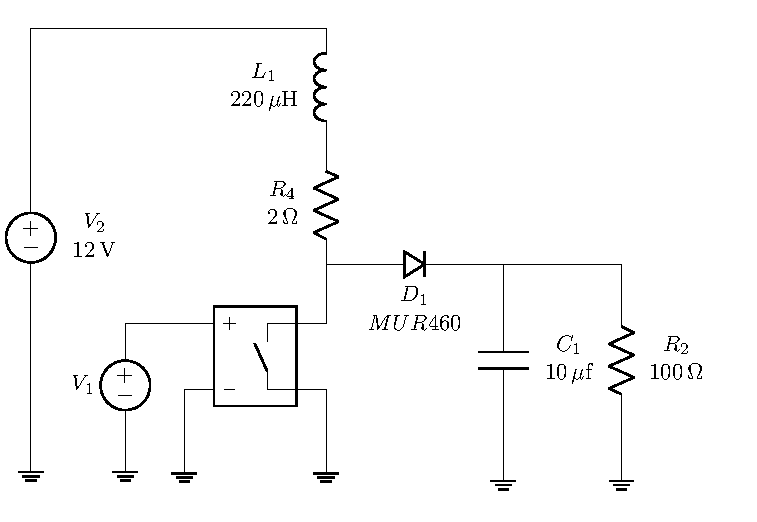
\includegraphics[width=0.8\linewidth, page=1]{ImagenesEjercicio-2/CircuitsEj2}
	\caption{Circuito de fuente Boost con llave ideal.}
	\label{fig:ej2:circuito}
\end{figure}

\subsection{Calculo del duty cycle}

Para el período de encendido, el hemicircuito es el siguiente. 

\begin{figure}[H]
	\centering
	\includegraphics[width=0.8\linewidth, page=2]{ImagenesEjercicio-2/CircuitsEj2}
	\caption{Circuito de fuente Boost con llave cerrada.}
	\label{fig:ej2:circuito_off}
\end{figure}

Planteando la mallas 1 y las corrientes en el nodo $A$ se obtienen las siguientes ecuaciones:
\begin{equation}
\begin{cases}
V_2 - L \dot{I_L} - R_4 I_L = 0 \\
C \dot{V_C} = -\frac{V_O}{R_2}
\end{cases}
\label{ej2:eq:on}
\end{equation}

Operando algebraicamente se obtienen las matrices: 
\begin{equation*}
\begin{gathered}
\mathbb{A}_{on} =  \begin{pmatrix}
	-R_4/L & 0 \\
	0 & -1/ C R_2
\end{pmatrix} \ \ \
\mathbb{B}_{on} =  \begin{pmatrix}
	1/L \\
	0
\end{pmatrix} \\
\mathbb{C}_{on} =  \begin{pmatrix}
	0 & 1 \\
\end{pmatrix}
\end{gathered}
\end{equation*}

Por otro lado, durante el apagado, el hemicircuito resultante es el que se muestra a continuación.

\begin{figure}[H]
	\centering
	\includegraphics[width=\linewidth, page=3]{ImagenesEjercicio-2/CircuitsEj2}
	\caption{Circuito de fuente Boost con llave cerrada.}
	\label{fig:ej2:circuito_on}
\end{figure}

De forma similar al caso anterior, planteando la malla externa y la suma de corrientes en el nodo $B$, se obtienen las ecuaciones siguientes:

\begin{equation}
\begin{cases}
V_2 - L \dot{I_L} - R_4 I_L - V_O = 0 \\
I_L = I_C + I_O = C\dot{V_C} + \frac{V_O}{R_2}
\end{cases}
\label{ej2:eq:off}
\end{equation}

Operando algebraicamente se obtienen las matrices: 
\begin{equation*}
\begin{gathered}
\mathbb{A}_{off} =  \begin{pmatrix}
	-R_4/L & -1/L \\
	1/C & -1/ C R_2
\end{pmatrix} \ \ \
\mathbb{B}_{off} =  \begin{pmatrix}
	1/L \\
	0
\end{pmatrix} \\
\mathbb{C}_{off} =  \begin{pmatrix}
	0 & 1 \\
\end{pmatrix}
\end{gathered}
\end{equation*}

Se definen las matrices $\mathbb{A}$, $\mathbb{B}$ y $\mathbb{C}$ de la forma:
\begin{equation*}
\mathbb{A} = \mathbb{A}_{on} \cdot d + \mathbb{A}_{off} \cdot (1-d) =  \begin{pmatrix}
	-R_4/L & (d-1)/L \\
	(1-d)/C & -1/ C R_2
\end{pmatrix}
\end{equation*}

\begin{equation*}
\mathbb{B} = \mathbb{B}_{on} \cdot d + \mathbb{B}_{off} \cdot (1-d) = \begin{pmatrix}
	1/L \\
	0
\end{pmatrix}
\end{equation*}

\begin{equation*}
\mathbb{C} = \mathbb{C}_{on} \cdot d + \mathbb{C}_{off} \cdot (1-d) = \begin{pmatrix}
	0 & 1
\end{pmatrix}
\end{equation*}

Finalmente, dado que la transferencia en el permanente esta dada por $H = -\mathbb{C} \cdot \mathbb{A}^{-1} \cdot \mathbb{B}$, se obtiene que:
\begin{equation*}
H = \frac{\left( 1 - d \right) R_2}{R_2 d^2 - 2 d R_2 + R_2 + R_4}
\end{equation*}
%H = \frac{\left( 1 - d \right) R_2}{R_2 d^2 - 2 d \left( R_2 + R_4 \right) + R_2 + R_4}

Reemplazando con $R_4 = 2 \ \Omega$, $R_2 = 100 \ \Omega$, y sabiendo que se busca que $H = V_o / V_2 = 2$, se obtienen dos resultados matemáticamente posibles, siendo estos $d = 0.544$ y $d = 0.956$. La aparición de dos valores se debe justamente a la consideración de los elementos parásitos en el circuito. La curva $\frac{V_o}{V_d}$ real se aleja de la ideal de manera decreciente. De los dos valores que se obtienen el segundo se descarta debido a que es el que se encuentra alejado de la fuente ideal, y se disipará una mayor potencia.

Por otro lado, utilizando la transferencia de la fuente Boost ideal, es decir sin $R_4$, se puede obtener que el duty cycle deseado es:
\begin{align*}
V_o &= \frac{V_2}{1 - d}	\\
1 - d &= \frac{V_2}{V_o} = \frac{12 \ V}{24 \ V} \\
d &= 0.5
\end{align*}

Este valor es cercano al obtenido considerando la alinealidad.

\subsection{Cálculos y simulaciones}

Se analizaron las señales propias del circuito. Considerando la fuente Boost ideal, se puede notar que la corriente en la bobina sigue siendo la misma, ya que agregar una resistencia en serie no cambia dicha variable. Es por ello que tanto la corriente como la tensión en el inductor se calculan de la misma forma, siendo así la corriente media en la bobina y su ripple:
\begin{equation*}
	I_{DC} = \frac{I_O}{1 - d} = \frac{V_O}{R_2 (1 - d)} = 526.137 \ mA
\end{equation*}
\begin{equation*}
	\Delta I_L = \frac{V_L}{L}\Delta t =  \frac{V_L}{L}  \frac{d}{f} = 494.404 \ mA  
\end{equation*}	% o 414.687 \ mA si usas (1 - d)

\begin{figure}[H]
	\centering
	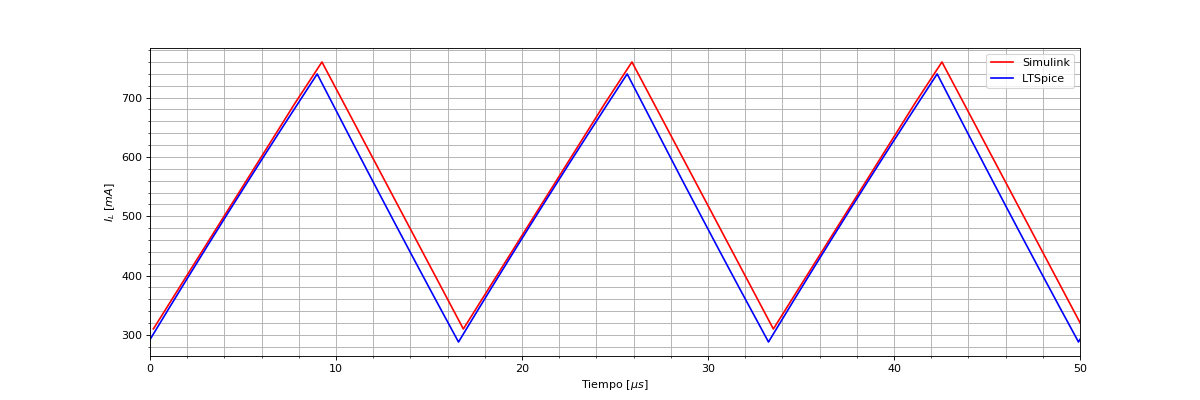
\includegraphics[width=\linewidth]{ImagenesEjercicio-2/il.png}
	\caption{Corriente sobre la bobina en el permanente.}
	\label{fig:ej2:il}
\end{figure}

Para la tensión, mientras la llave se mantenga cerrada
\begin{equation*}
	V_L = V_S = 12 \ V
\end{equation*}

y mientras se mantenga abierta
\begin{equation*}
	V_L = V_S - V_O = 12 \ V - 24 \ V = -12 \ V
\end{equation*}

\begin{figure}[H]
	\centering
	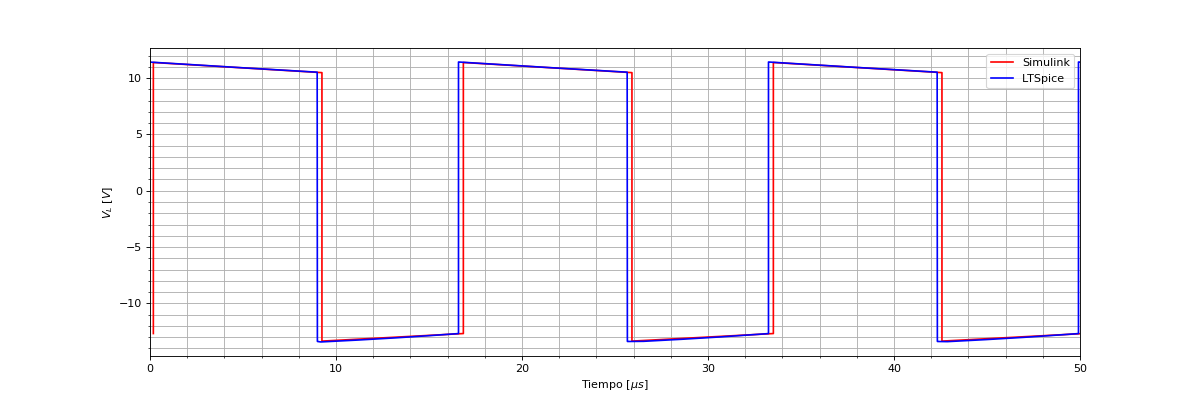
\includegraphics[width=\linewidth]{ImagenesEjercicio-2/vl.png}
	\caption{Tensión sobre la bobina en el permanente.}
	\label{fig:ej2:vl}
\end{figure}
vale la pena mencionar que en el Gráfico (\ref{fig:ej2:vl}) las tensiones no son exactamente 12 y -12, esto se debe a la caída de potencial sobre la $R_{2}$ y la tensión de forward $V_d$.\\
Para el diodo, al no ser ideal, se debe considerar la corriente en reversa. Esta se hace presente al llevar al estado de no conducción al diodo, es decir, esta se da unos instantes al cerrar la llave cuando se pone el ánodo a tierra. Cabe aclarar que el modelo del diodo existente en Simulink no considera la corriente en inversa $I_{RR}$.

\begin{figure}[H]
	\centering
	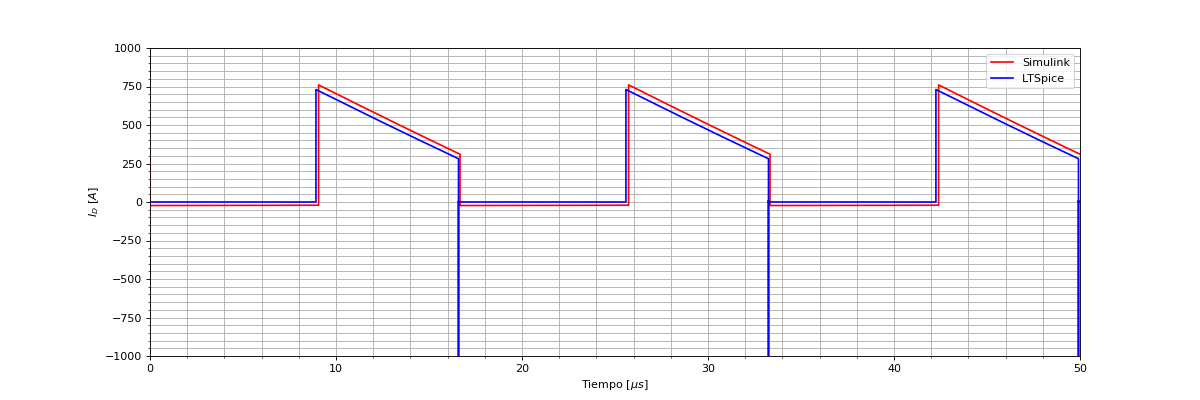
\includegraphics[width=\linewidth]{ImagenesEjercicio-2/id.png}
	\caption{Corriente sobre el diodo en el permanente.}
	\label{fig:ej2:id}
\end{figure}

Finalmente, se calcula la tensión de salida. Si bien esta debería ser constante (ya que se asumió que la corriente lo es) no es así. Dado que la corriente media en el capacitor es nula, la corriente media en la carga es la misma que la de la bobina. Como esta última posee un ripple, también existirá una variación en la carga. Observando la corriente del capacitor, se puede calcular la variación de tensión de la forma:

\begin{align*}
I_O \ d \ T_S &= C \Delta V_O	\\
\Delta V_O &= \frac{I_O d}{C f} = 0.747 \ V
\end{align*}

\begin{figure}[H]
	\centering
	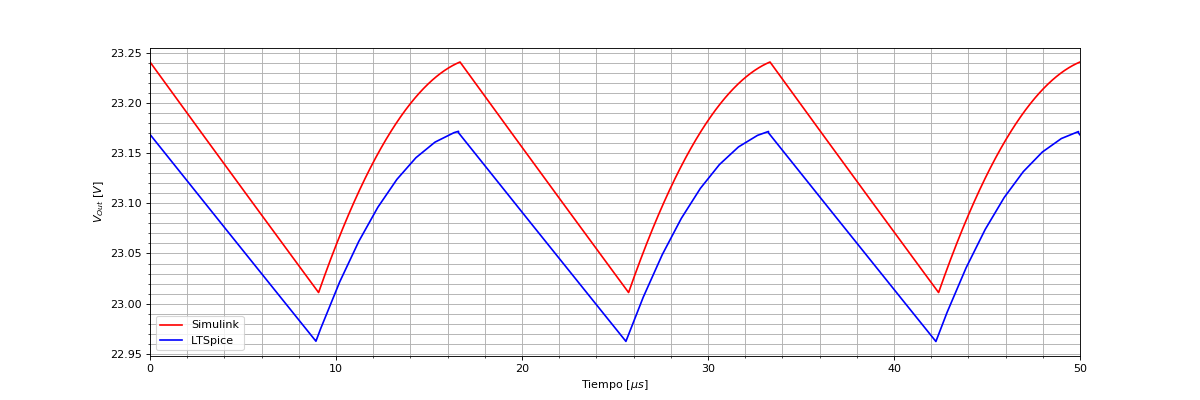
\includegraphics[width=\linewidth]{ImagenesEjercicio-2/vout.png}
	\caption{Tensión sobre la salida en el permanente.}
	\label{fig:ej2:vout}
\end{figure}

Además es posible observar que:

\begin{equation*}
\frac{\Delta V_O}{V_O} \% = \frac{0.747 \ V}{24 \ V} \cdot 100 \% = 1.987 \%
\end{equation*}

\subsection{Conclusión de los datos obtenidos}

Se simuló el circuito tanto en Simulink como en LTSpice. Se observa que la tensión media a la salida es menor a la que se requería. Esto se debe a que en los cálculos planteados en las Ecuaciones (\ref{ej2:eq:on}) y (\ref{ej2:eq:off}) se considera al diodo como uno ideal.

Simulando nuevamente con un diodo ideal, se nota que la tensión de salida es más adecuada a la calculada.

\begin{figure}[H]
	\centering
	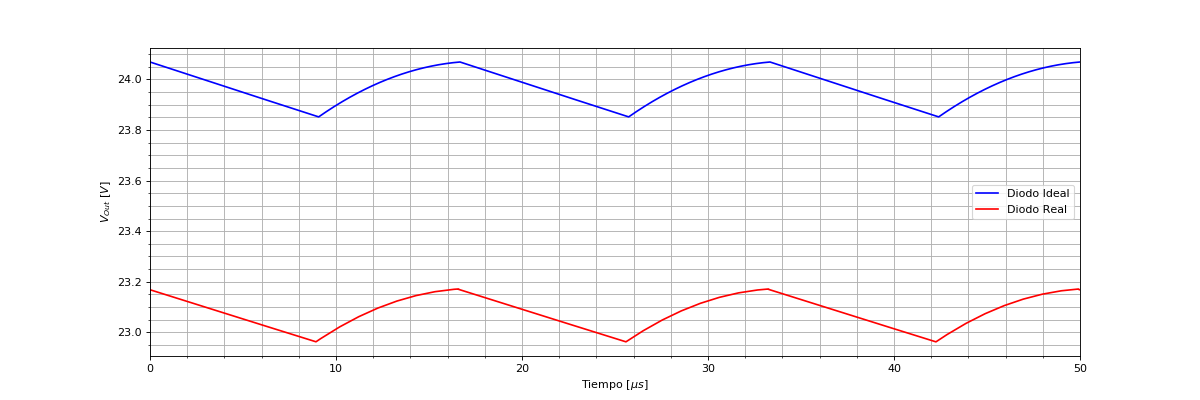
\includegraphics[width=\linewidth]{ImagenesEjercicio-2/vo_diodo_ideal.png}
	\caption{Tensión sobre la salida en el permanente con diodo ideal.}
	\label{fig:ej2:vo_diodo_ideal}
\end{figure}
Para la simulación de LTSpice se retocó el valor de duty cycle a un valor tal que cumpla las especificaciones, siendo este valor $D=0.56225$ obteniendo las siguientes curvas:
\begin{figure}[H]
	\centering
	%vo_diodo_ideal_sim
	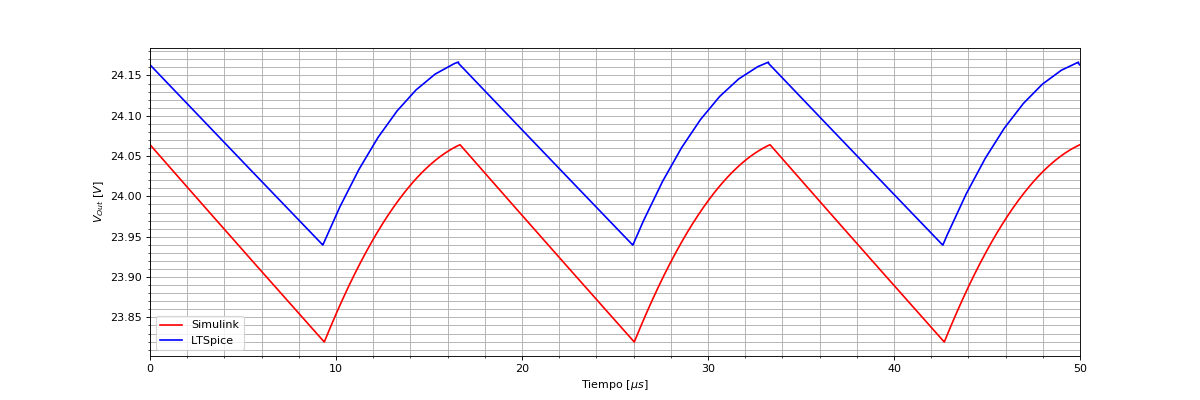
\includegraphics[width=\linewidth]{ImagenesEjercicio-2/vo_duty_ideal.png}
	\caption{Tensión sobre la salida en el permanente con diodo ideal en Matlab y DT ajustado LTSpice.}
	\label{fig:ej2:vo_diodo_ideal_ltspice}
\end{figure}

Finalmente, cabe hacer una aclaración con respecto a las curvas observadas en la Figura (\ref{fig:ej2:id}). En dicho gráfico se nota que la corriente $I_{RR}$ del diodo llega a valores elevados. Esto se debe a la idealización de la llave empleada en las simulaciones. Esto se analiza en mayor profundidad en la siguiente sección.

%\end{document}
